\cotefile{63}

\scanpage{4}\mspage{1}
\begingroup
\makeatletter\tagsleft@true\makeatother
1. \uline{Generalized} \uline{Weierstrass} \uline{form}. Let $E$ be an elliptic curve defined over a field - $K$ with a $K$-rational point $O$. In the projective embedding defined by $3O$ the curve can be written in the form
\[
y^2+a_1xy+a_3y=x^3+a_2x^2+a_4x+a_6
\qquad \unsure{\ldotp|,}\quad\unsure{,}\quad a_i\in K
\tag*{(1.1)}
\]

Put
\[
\begin{aligned}
 b_2&=a_1^2+4a_2                  & c_4&=b_2^2-24b_4\\
 b_4&=a_1a_3+2a_4                  & c_6&=-b_2^3+36b_2b_4-216b_6\\
 b_6&=a_3^2+4a_6                    & \Delta&=-b_2^2b_8-8b_4^3-27b_6^2+9b_2b_4b_6\ne0\\
 b_8&=a_1^2a_6-a_1a_3a_4+4a_2a_6+a_2a_3^2-a_4^2
                                      & j&=c_4^3/\Delta
\end{aligned}
\tag*{(1.2)}
\]

These quantities are related by
\[
4b_8=b_2b_6-b_4^2 \qquad 1728\Delta=c_4^3-c_6^2
\tag*{(1.3)}
\]

A differential of first kind is given by
\[
\omega=\frac{dx}{2y+a_1x+a_3}
=\frac{dx}{F_y(x,y)}=-\frac{dy}{F_x(x,y)}
=\frac{dy}{3x^2+2a_2x+a_4-a_1y},
\tag*{(1.4)}
\]
where we have put
\[
F(X,Y)=Y^2+a_1XY+a_3Y-X^3-a_2X^2-a_4X-a_6.
\tag*{(1.5)}
\]

Putting
\[
\eta=y+\frac{a_1x+a_3}{2}\qquad\text{and}\qquad
\xi=x+\frac{b_2}{12},
\tag*{(1.6)}
\]
the equation (1.1) becomes
\[
\eta^2=x^3+\frac{b_2}{4}x^2+\frac{b_4}{2}x+\frac{b_6}{4}
=\xi^3-\frac{c_4}{48}\xi-\frac{c_6}{864}.
\tag*{(1.7)}
\]

Thus the relation with Weierstrass is given by
\[
\begin{aligned}
\xi&=\wp(u) & c_4&=12g_2 &
\omega&=\frac{d\xi}{2\eta}=du\\
2\eta&-\wp'(u) & c_6&=216g_3
\end{aligned}
\tag*{(1.8)}
\]
\endgroup

% archive sheet number: 3

\scanpage{5}\mspage{2}
\begingroup
\makeatletter\tagsleft@true\makeatother
2. \uline{Change} \uline{of} \uline{coordinates}. Suppose $E':\quad y^{\prime\,2}+a_1'x'y'+\ldotp\,\ldotp\,\ldotp\,\ldotp$ is another curve of the same type as $E$, and $f:E'\overset{\sim}{\longrightarrow}E$ an isomorphism over $K$. carrying $O'$ into $O$. Then there are $r,s,t$ and $u\ne0$ in $K$ such that
\[
\begin{aligned}
x\circ f&=u^2x'+r & \omega\circ f&=u^{-1}\omega'.\\
y\circ f&=u^3y'+su^2x'+t
\end{aligned}
\tag*{(2.1)}
\]

The coefficients $a_i'$ are related to the $a_i$ \deleted{\illegible{1}} and the $b_i'$ to the $b_i$ by the formulas:
\begingroup\scriptsize
\[
\begin{aligned}
ua_1'&=a_1+2s & u^8b_8'&=b_8+3rb_6+3r^2b_4+r^3b_2+3r^{\unsure{4}}\\
u^2a_2'&=a_2-sa_1+3r-s^2 & u^6b_6'&=b_6+2rb_4+r^2b_2+4r^3\\
u^3a_3'&=a_3+ra_1+2t=F_y(r,t) & u^4b_4'&=b_4+rb_2+6r^2\\
u^4a_4'&=a_4-sa_3+2ra_2-(t+rs)a_1+3r^2-2st
 & u^2b_2'&=b_2+12r.\\
 &= -F_x(r,t)-sF_y(r,t)\\
u^6a_6'&=a_6+ra_4+r^2a_2+r^3-ta_3-t^2-rta_1\\
 &= -F(r,t)
\end{aligned}
\tag*{(2.2)}
\]
\endgroup

From these we check that:
\[
u^4c_4'=c_4\qquad u^6c_6'=c_6\qquad
u^{12}\Delta'=\Delta\qquad j'=j.
\tag*{(2.3)}
\]

\uline{Example} \unsure{`|``}generic $E_j$''. The equation
\[
y^2+xy=x^3-\frac{36}{j-1728}x-\frac{1}{j-1728}
\tag*{(2.4)}
\]
has $c_4=c_6=\dfrac{j}{j-1728}$ and $\Delta=\dfrac{j^2}{(j-1728)^3}$. Hence for $j\ne0,1728$ it gives a curve with invariant '$j$.

Using the formulas above, it is easy to show that $j$ can be arbitrary in $K$, and that for $K$ algebraically closed, two $E$'s with the same $j$ are \unsure{isomorphic} It is also easy to compute the group of automorphisms (but not, alas, the ring of endomorphisms). See Serre's ``Courbes Elliptiques - Formulaire'' for the details.
\endgroup

% archive sheet number: 4

\scanpage{6}\mspage{3.}
3. \uline{The} ``\uline{minimal}'' \uline{Weierstrass} \uline{equations} \uline{over} \uline{a} \uline{valuation} \uline{ring}. Let $v$ be a discrete valuation of $K$, with valuation ring $R$, prime ideal $\mathfrak{p}$, and residue field $k=R/\mathfrak{p}$. Let $E$ be an elliptic curve over $K$, with a $K\cdot$rational point $O$.

\uline{Defn 3.1}: An equation for $E$ of the form (1.1) is minimal (with respect to $v$) if $v(a_i)\geqslant0$ for all $i$ and if $v(\Delta)$ is minimal, subject to that condition.

\uline{Theorem 3.2}\unsure{.|:} \uline{A} \uline{minimal} \uline{equation} \inserted{for $E$} \uline{exists}, \uline{and} \uline{is} \uline{unique} \uline{up} \uline{to} \uline{a} \uline{change} \uline{of} \uline{coördinates} \uline{of} \uline{the} \uline{form} (2.1) \uline{with} $r,s,t\in R$ \uline{and} $u$ \uline{invertible} \uline{in} $R$.

Existence is obvious. Let $y^{\prime\,2}+a_1'x'y'+\unsure{\ldotp\,\ldotp|\ldots}$ and $y^2+a_1xy+\ldots$ be two minimal equations for the same $E$. Since $\Delta\ne0$ and $v(\Delta')=v(\Delta)$ we conclude from\deleted{\illegible{1}} (2.3) that $v(u)=0$. Now from the transformation of $b_8$ and $b_6$ in (2.2) we see that $3r\in R$ and $4r\in R$, hence $r\in R$. \inserted{Next} The transformation of $a_2$ shows that $s\in R$, and that of $a_6$ shows that $t\in R$.

\uline{Corollary 3.3:} \uline{The} \uline{differential} $\omega$ \uline{associated} \uline{with} \uline{a} \uline{minimal} \deleted{Weierstrass form} \uline{is} \uline{unique} \uline{up} \uline{to} \uline{a} \uline{unit} \uline{in} $R$.

\uline{Remarks}: 1) If $a_i\in R$ and $v(\Delta)<12$, then the equation (1.1) is automatically minimal. The converse is true if $j\in R$ and $p=\operatorname{char}k\ne2,3$. A complete algorithm for reducing to minimal form in all \unsure{cases|\deleted{c}cases} is given below.

2) Let $\mathscr{M}$ be a collection of discrete valuations of $K$. For each $v\in\mathscr{M}$, let $y_v^2+a_{1,v}x_vy_v+\ldotp\,\ldotp\,\ldotp\,\ldotp$ be a minimal equation for $E$ relative to $v$, with corresponding differential $\omega_v$ and discriminant $\Delta_v$. Then the ``divisor'' $\displaystyle \mathfrak{d}_E=\sum_{v\in\mathscr{M}}v(\Delta_v)v$ should be regarded as \uline{the} \uline{discriminant} \uline{of} $E$.

Let $F(x,y)=y^2+a_1xy+\ldots$ be an arbitrary Weierstrass equation for $E$ over $K$, and let $\omega_F$ and $\Delta_F$ be the corresponding differential and discriminant. Then the \uline{class} of the divisor $\displaystyle \mathfrak{u}_F=\sum_v v\left(\frac{\omega}{\omega_v}\right)v$ is independent of $F$, and we have $12\mathfrak{u}_F=\mathfrak{d}_E-(\Delta_F)$, so that $12\mathfrak{u}_F\sim\mathfrak{d}_E$.

3) In case $\mathscr{M}$ is the set of valuations associated with a principal ideal domain $D$ with field of fractions $K$, then it is easy to see that we can find one equation $F$ which simultaneously minimal for all $v$, so that $\mathfrak{u}_F=0$, and $\mathfrak{d}=(\Delta_F)$.

4) If $j\in R$, then $\Delta$ divides $c_4^3$ and $c_6^2$. From (1.7) we see that if $48\mathfrak{p}^4\mid c_4$ and $864\mathfrak{p}^6\mid c_6$, then the equation is not minimal. Hence \uline{if} $j\in R$ \uline{and} \uline{equation} \uline{minimal} \uline{we} \uline{have} $v(\Delta)<$ \deleted{\illegible{?}} $12+12v(2)+6v(3)$

% archive sheet number: 5

\scanpage{7}\mspage{4.}
\begingroup
\makeatletter\tagsleft@true\makeatother
4. \uline{The} \uline{canonical} \uline{filtration} \uline{on} \uline{the} \uline{group} of $v$-\uline{adic} \uline{points}. Let $F(x,y)-y^2+a_1xy+\ldotp$ be a minimal equation for $E$ relative to a valuation $v$. Let $\widetilde F(x,y)$ be the reduction of $F$ $(\bmod\,\mathfrak{p})$ and let $\widetilde E$ denote the plane cubic $\widetilde F=0$ defined over the residue field $k$. By Theorem 3.2, $\widetilde E$ is uniquely determined by $E$ up to a projective transformation of the form (2.1) over $k$: Let $\widetilde E_0$ denote the non-singular part of $\widetilde E$. Then $\widetilde E_0$ is an algebraic group with origin $\widetilde O$. (If $\widetilde E$ is non singular, then $\widetilde E_0-\widetilde E$ is an elliptic curve, If $\widetilde E$ has a node
\parbox[c]{1.4em}{\setlength{\topsep}{0pt}\figure{
\begin{tikzpicture}[x=0.95em,y=0.95em]
\draw[line width=.8pt,line cap=round] (0.97,.01) .. controls (.73,.19) and (.45,.66) .. (.24,.64) .. controls (.01,.65) and (-.02,.30) .. (.12,.16) .. controls (.29,.02) and (.49,.18) .. (.60,.34) .. controls (.76,.52) and (.85,.69) .. (.96,.87);
\end{tikzpicture}}}, then $\widetilde E_0\approx\mathbb{P}^1-(\text{two points})$ is a multiplicative group, and if $\widetilde E$ has a cusp
\parbox[c]{1.4em}{\setlength{\topsep}{0pt}\figure{
\begin{tikzpicture}[x=0.95em,y=0.95em]
\draw[line width=.9pt,line cap=round] (.91,.66) .. controls (.81,.40) and (.59,.24) .. (.02,.22) .. controls (.61,.23) and (.87,.25) .. (1.01,.02);
\end{tikzpicture}}}, then $\widetilde E_0=\mathbb{P}^1-(\text{one point})$ is an additive group; here We have ignored questions of rationality, but if $k$ is perfect, so that the singularity of $\widetilde E$ is rational over $k$, then the analysis is the same, except that in case of a node, $\widetilde E_0$ is a multiplicative group ``twisted'' by the quadratic extension obtained by adjoining to $k$ the two tangents at the node)

Let $E(K)$ denote the group of points on $E$ rational over $K$, and let $\rho:E(K)\longrightarrow\widetilde E(k)$ denote the reduction map (defined naively in terms of the given projective coordinates --- by Theorem 3.2 it is independent of the coörds.) Let $E_0(K)=\rho^{-1}(\widetilde E_0(k))$ be the set of points whose reduction is non-singular.

\uline{Theorem 4.1}: $E_0(K)$ \uline{is} \uline{a} \uline{subgroup} \uline{of} \uline{finite} \uline{index} \uline{in} $E(K)$, \uline{and} $\rho_0:E_0(K)\to\widetilde E_0(k)$ \uline{is} \uline{a} \uline{homomorphism} \uline{of} \uline{groups}.

A straightforward but tedious proof can be given, using the addition formulae, for everything except the `finite index''. That finiteness depends on the minimality of the equation, and a proof of finiteness is implicit in the algorithm for reducing to minimal form given below.

We denote the kernel of $\rho_0$ by $E_1(K)$; it consists of the points $P=(x,y)$ in $E(K)$ such that $v(x)<0$ and $v(y)<0$. Clearly, from \unsure{(1 1)|(1.1)} since $v(a_i)\geqslant0$, we have $v(x)<0\Longleftrightarrow v(y)<0$, in which case $v(x)=-2m$ and $v(y)=-3m$ for some $m$. For each $m\geqslant1$ we let $E_m(K)=\{(x,y)\in E(K)\mid v(x)\leq-2m\ \text{and}\ v(y)\leq-3m\}$ (understanding of course that $O\in E_m(K)$ for all $m$).

\uline{Theorem 4.2}: \uline{Let} $z=-\dfrac{x}{y}$. \uline{Then} $z$ \uline{is} \uline{a} \uline{uniformising} \uline{parameter} \uline{at} $O$. \uline{The} \uline{expansions}
\begingroup\scriptsize
\[
\begin{aligned}
x&=z^{-2}-a_1z^{-1}-a_2-a_3z-(a_4+a_1a_3)z^2
 -\ldotp\,\ldotp\,\ldotp\,\ldotp\\
y&=-z^{-1}x=-z^{-3}+a_1z^{-2}+a_2z^{-1}+a_3+(a_4+a_1a_3)z+\ldots\\
\omega&=dt\bigl(1+a_1t+(a_1^2+a_2)t^2+(a_1^3+2a_1a_2+a_3)t^3+
 (a_1^4+3a_1^2a_2+6a_1a_3+a_2^2+2a_4)t^4+\ldotp\,\unsure{-|\ldotp}
\end{aligned}
\tag*{(4.3)}
\]
\endgroup
\uline{have} \uline{coefficients} \uline{in} $R$. \uline{So} \uline{also} \uline{does} \uline{the} \uline{formal}
\deleted{$(\unsure{a_1^4+3a_1^2a_2}+6a_1\unsure{a_3}\unsure{+a_2^2+2a_4})\unsure{t^4}$}
\uline{group} \uline{law} $\Phi(Z_1,Z_2)=Z_1+Z_2+\ldotp\,\ldotp\,\ldotp\,\ldotp$ \uline{defined} \uline{by} \uline{the} \uline{equation} $z(P+Q)=\Phi(z(P),z(Q))$. \uline{If} $R$ \uline{is} \uline{complete}, \uline{then} \uline{the} \uline{map} $z\longmapsto(x(z),y(z))$, \uline{for} $z\in\mathfrak{p}$, \uline{gives} \uline{an} \uline{isomorphism} \uline{of} $\mathfrak{p}_{\Phi}$ (\uline{the} \uline{prime} \uline{ideal} \uline{endowed} \uline{with} \uline{group} \uline{structure} \uline{via} $\Phi$) \uline{onto} $E_1(K)$, \uline{under} \uline{which} \uline{the} \uline{subgroups} $\mathfrak{p}^m_{\Phi}$ \uline{correspond} \uline{to} $E_m(K)$ \uline{for} \uline{all} $m\geqslant1$.
\endgroup

% archive sheet number: 6

\scanpage{8}\mspage{5}
\begingroup
\makeatletter\tagsleft@true\makeatother
The proof is straightforward. Let $z=\dfrac{x}{-y}$, $w=\dfrac{1}{-y}$, so that $x=\dfrac{z}{w}$ and $y=-\dfrac{1}{w}$. Then in terms of $w$ and $z$ the equation for $E$ is
\[
 w(1-a_1z-a_3w)=z^3+a_2z^2w+a_4zw^2+a_6w^3.
 \tag*{(4.4)}
\]
This shows that we have
\begingroup\scriptsize
\[
\begin{aligned}
w&=z^3+a_1z^4+(a_1^2+a_2)z^5+(a_1^3+2a_1a_2+a_3)z^6+
 (a_1^4+3a_1^2a_2+3a_1a_3+a_2^2+a_4)z^7+\ldots\\
 &=z^3+A_1z^4+A_2z^5+\ldots
\end{aligned}
\tag*{(4.5)}
\]
\endgroup
where $A_\nu$ is a polynomial of weight $\nu$ in the $a_i$ with positive integral coeffs Hence the expansions of $y=-\dfrac{1}{w}$ and $x=-zy$ in terms of $z$ have coefficients in $\mathbb{Z}[a_1,a_2,a_3,a_4,a_6]$. Now
\[
 \frac{\omega}{d\deleted{\unsure{t}}z}=
 \frac{dx/d\deleted{\unsure{t}}z}{2y+a_1x+a_3}=
 \frac{-2\deleted{\unsure{t}}z^{-3}+\ldotp}{-2\deleted{\unsure{t}}z^{-3}+\ldotp}=
 \frac{dy/d\deleted{\unsure{t}}z}{3x^2+2a_2x+a_4-a_1y}=
 \frac{3z^{-4}+\ldotp}{3z^{-4}+\ldots}
\]
has coefficients in $\mathbb{Z}[\frac{1}{2},a_1,\ldots,a_6]$ but also in $\mathbb{Z}[\frac{1}{3},a_1,\ ,a_6]$, hence in $\mathbb{Z}[a_1,\ ,a_6]$. As for the group law, if $z_1$ and $z_2\in\mathfrak{p}$, then the line joining the points $(z_1,w_1)$, $(z_1,w_2)$ in the $(z,w)$-plane has slope $\in\mathfrak{p}^2$, because
\[
 \frac{w_2-w_1}{z_2-z_1}=
 \frac{z_2^3-z_1^3}{z_2-z_1}
 +A_1\frac{z_2^4-z_1^4}{z_2-z_1}+
\]
\margin{\unsure{with|the} $A_i$ as above in (\unsure{4}.5)}
Call this slope $\lambda=\lambda(z_1,z_2)=z_2^2+z_1z_2+z_1^2+A_1(z_2^3+z_2^1z_1+z_1z_1^2+z_1^3)+\unsure{\ldotp\,\ldotp|\ldots}$. Put $\nu=\nu(z_1,z_2)=w_i-\lambda z_i$ $(i=1,2)$. Substituting $w=\lambda(z_1,z_2)z+\nu(z_1,z_2)z$ in (4.4) we find a cubic in $z$ with roots $w_1$ and $w_2$. Looking at the sum of the roots, one sees that the third root $\deleted{\unsure{t}}z_3$ is expressed as a power series in $z_1,z_2$ with coeffs in $R$. In fact,
\[
 z_1+z_2+z_3=
 \frac{a_1\lambda+a_3\lambda^2-a_2\nu-2a_4\lambda\nu-3a_6\lambda^2\nu}
 {1+a_2\lambda+a_4\lambda^2+a_6\lambda^3}
 \tag*{(4.6)}
\]
\margin{(sauf erreur)}
Thus we have the `canonical filtration''
\[
 E(K)\supset E_0(K)\supset E_1(K)\supset E_2(K)\supset\ldots
 \qquad\supset(O)=\bigcap_{m=1}^{\infty}E_m(K)
 \tag*{(4.7)}
\]
with quotients
\begingroup\small
\[
 E(K)\big/E_0(K)\quad\text{finite},\qquad
 E_0\big/E_1\mathrel{\deleted{\unsure{\subset}}\hookrightarrow}\widetilde E_0(k),
 \quad\text{and}\quad E_m\big/E_{m+1}\hookrightarrow k^+
 \quad\text{for }m\geqslant1.
\]
\endgroup
Of course the inclusions $\hookrightarrow$ are bijections $\overset{\sim}{\to}$ if $R$ is complete.
\endgroup

% archive sheet number: 7

\scanpage{9}\mspage{6}
\begingroup
\makeatletter\tagsleft@true\makeatother
5. \uline{Application}: \uline{The} \uline{relation} \uline{between} $L_v(1)$ \uline{and} $\int_{E_v}|\omega_v|$ \uline{in} \uline{case} $k$ \uline{is} \uline{finite}.

Suppose now $R$ is complete and $k$ is finite with $q=\operatorname{Card} k$. On $K$ we agree to use the additive Haar measure with respect to which $R$ has measure $1$. This being agreed, a differential \inserted{$\omega$} on $E$ gives us a measure $|\omega|$ on $E(K)$ in the usual manner.

\uline{Corollary 5.1} (\unsure{of|cf} theorem 4.2) $\displaystyle\int_{E_1(K)}|\omega|=\frac{1}{q}$, if $\omega$ \uline{is} \uline{a} \uline{differential} \uline{of} $1^{\mathrm{st}}$ \uline{kind} \uline{on} $E$ \uline{coming} \uline{from} \uline{a} \uline{minimal} \uline{equation}.

Indeed, by (4.2) we have $\displaystyle\int_{E_1(K)}|\omega|=\int_{\mathfrak p}|dz|=\frac{\int_R|dz|}{(R:\mathfrak p)}=\frac{1}{q}$

The local factor occuring in the Euler product with a good functional equation is (Serre tells me) as follows, in which $N_v=\operatorname{Card}(\widetilde E_0(k))$\unsure{:|;|.}
{\small
\[
L_v(s)=\left\{
\begin{array}{@{}c@{\quad}l@{}}
\dfrac{1}{1-(q+1-N_v)q^{-s}+q^{1-2s}}
 & \parbox{.39\linewidth}{, if $\widetilde E$ non singular}\\[1.0ex]
\dfrac{1}{1-q^{-s}}
 & \parbox{.39\linewidth}{, if $\widetilde E$ has a node with the two tangents ratl over $k$ (in which case $N_v=q-1$, and $\widetilde E_0$ is the multiplicative group.)}\\[1.0ex]
\dfrac{1}{1+q^{-s}}
 & \parbox{.39\linewidth}{, if $\widetilde E$ has a node with irrational tangents (in which case $N_v=q+1$, and $\widetilde E_0$ is the twisted mult. group)}\\[1.0ex]
1 & \parbox{.39\linewidth}{, if $\widetilde E$ has a cusp (in which case $N_v=q$, and $\widetilde E_0$ is the additive gp.)}
\end{array}\right.
\tag*{(5.2)}
\]
}

In all cases therefore, $L_v(1)=\dfrac{q}{N_v}$. Since $N_v=(E_0(K):E_1(K))$: it follows from cor 5.1 that we have $\displaystyle\int_{E_0(K)}|\omega|=(L_v(1))^{-1}$, because $|\omega|$ is invariant under translation. Finally then,

\uline{Theorem 5.2}: \uline{If} \uline{we} \uline{use} \uline{the} \uline{measure} \uline{on} $K$ \uline{for} \uline{which} $R$ \uline{gets} \uline{measure} $1$, \uline{and} \uline{use} \uline{a} \uline{differential} \uline{of} \uline{first} \uline{kind} $\omega$ \uline{coming} \uline{from} \uline{a} \uline{minimal} \uline{equation}, \uline{then}
\[
\int_{E(K)}|\omega|=\frac{(E(K):E_0(K))}{L_v(1)}
\tag*{(5.3)}
\]
In other words, the ``fudge factors''\ of Birch and Sw-Dyer are just the indices $(E(K):E_0(K))$,
\endgroup

% archive sheet number: 8

\scanpage{10}\mspage{\unsure{7|9}.}
6. \uline{The} \uline{Neron} \uline{minimum} \uline{model}. Suppose $k$ algebraically closed. One can find a regular scheme $X$ over $R$ such that $X\underset{R}{\times}K\approx E$ and such that $X$ is ``minimal'' relative to the map $X\longrightarrow\operatorname{Spec} R$ (i.e such that that map cannot be factored $X\longrightarrow X'\longrightarrow\operatorname{Spec} R$ in such a way that $X\underset{R}{\times}K\to X'\underset{R}{\times}K$ is an isomorphism. Such an $X$ is unique up to isom. Its fiber $\widetilde X=X\underset{R}{\times}k$ is of one of the following types

\diagram{%
\setlength{\arraycolsep}{2.7pt}\renewcommand{\arraystretch}{1.35}%
\resizebox{\linewidth}{!}{$%
\begin{array}{|l|*{10}{c|}}
\hline
\text{\deleted{\unsure{Kodaira} symbol}} &
\deleted{\mathrm I_0} &
\deleted{\mathrm I_{\unsure{0|b|\nu}}^{\unsure{*|\nu}}} &
\deleted{\mathrm I_{\unsure{b|0}}} &
\multicolumn{7}{l|}{\deleted{\mathrm I_{\unsure{b|0}}^{*}}}\\ \hline
\makebox[46mm][l]{Kodaira symbol} &
\makebox[18.2mm]{$\mathrm I_0$} &
\makebox[18.2mm]{$\mathrm I_{\nu}\;(\nu>0)$} &
\makebox[18.2mm]{$\mathrm{II}$} &
\makebox[18.2mm]{$\mathrm{III}$} &
\makebox[18.2mm]{$\mathrm{IV}$} &
\makebox[18.2mm]{$\mathrm I_0^{*}$} &
\makebox[18.2mm]{$\mathrm I_\nu^{*}\;(\nu>0)$} &
\makebox[18.2mm]{$\mathrm{IV}^{*}$} &
\makebox[18.2mm]{$\mathrm{III}^{*}$} &
\makebox[18.2mm]{$\mathrm{II}^{*}$} \\ \hline
\shortstack[l]{Picture\\(the numbers\\indicate multi-\\plicities)} &
\parbox[c][5.45cm][c]{1.82cm}{\figure{%
\begin{tikzpicture}[x=.0158cm,y=-.0158cm,line width=.8pt,line cap=round,line join=round,every node/.style={inner sep=0pt,font=\scriptsize}]
\path[use as bounding box] (0,0) rectangle (112,318);
\draw (51,59) .. controls (77,44) and (79,73) .. (77,130) .. controls (77.6,165.4) and (75.68,195.4) .. (70.808,215.248);
\draw[line width=.4pt,opacity=.3] (70.808,215.248) -- (70.3,217.2);
\draw (68.469,223.093) .. controls (65.552,231.181) and (61.8,235.72) .. (57,237) .. controls (33,246) and (26,216) .. (29,169) .. controls (30,122) and (38,65) .. (51,59);
\node at (88,146) {$1$};
\end{tikzpicture}}} &
\parbox[c][5.45cm][c]{1.82cm}{\figure{%
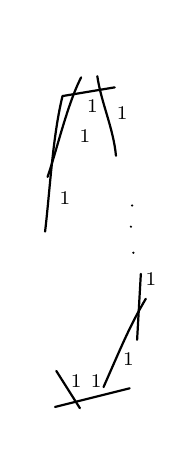
\begin{tikzpicture}[x=.0158cm,y=-.0158cm,line width=.8pt,line cap=round,line join=round,every node/.style={inner sep=0pt,font=\scriptsize}]
\path[use as bounding box] (0,0) rectangle (112,318);
\draw (14,164) .. controls (18,130) and (20,88) .. (28,55);
\draw (16,120) .. controls (23,100) and (32,61) .. (43,40);
\draw (28,55) -- (70,48);
\draw (56,39) .. controls (59,60) and (69,81) .. (71,103);
\draw (91,198) -- (88,251);
\draw (61,289) .. controls (76,255) and (82,240) .. (95,218);
\draw (22,305) -- (82,290);
\draw (23,276) -- (42,306);
\node at (30,137) {$1$};
\node at (46,87) {$1$};
\node at (52,63) {$1$};
\node at (76,69) {$1$};
\node at (99,202) {$1$};
\node at (81,267) {$1$};
\node at (55,284) {$1$};
\node at (39,284) {$1$};
\fill (84,143) circle[radius=.45pt];
\fill (83,160) circle[radius=.45pt];
\fill (85,181) circle[radius=.45pt];
\end{tikzpicture}}} &
\parbox[c][5.45cm][c]{1.82cm}{\figure{%
\begin{tikzpicture}[x=.0158cm,y=-.0158cm,line width=.8pt,line cap=round,line join=round,every node/.style={inner sep=0pt,font=\scriptsize}]
\path[use as bounding box] (0,0) rectangle (112,318);
\draw (30,70) .. controls (48,107) and (51,128) .. (53,170) .. controls (52,133) and (53,110) .. (74,69);
\node at (78,90) {$1$};
\end{tikzpicture}}} &
\parbox[c][5.45cm][c]{1.82cm}{\figure{%
\begin{tikzpicture}[x=.0158cm,y=-.0158cm,line width=.8pt,line cap=round,line join=round,every node/.style={inner sep=0pt,font=\scriptsize}]
\path[use as bounding box] (0,0) rectangle (112,318);
\draw (31,76) .. controls (46,108) and (53,124) .. (53,140) -- (53,183) .. controls (53,203) and (43,220) .. (32,235);
\draw (71,76) .. controls (58,110) and (53,125) .. (53,140) -- (53,183) .. controls (53,204) and (60,226) .. (75,241);
\node at (28,99) {$1$};
\node at (78,93) {$1$};
\end{tikzpicture}}} &
\parbox[c][5.45cm][c]{1.82cm}{\figure{%
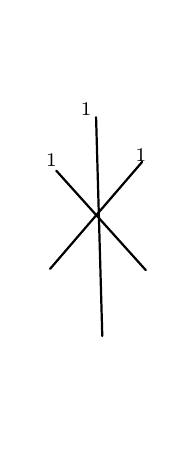
\begin{tikzpicture}[x=.0158cm,y=-.0158cm,line width=.8pt,line cap=round,line join=round,every node/.style={inner sep=0pt,font=\scriptsize}]
\path[use as bounding box] (0,0) rectangle (112,318);
\draw (55,72) -- (60,248);
\draw (23,115) -- (95,195);
\draw (92,108) -- (18,194);
\node at (47,66) {$1$};
\node at (19,107) {$1$};
\node at (91,103) {$1$};
\end{tikzpicture}}} &
\parbox[c][5.45cm][c]{1.82cm}{\figure{%
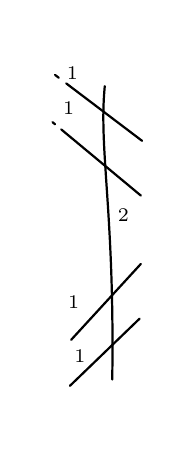
\begin{tikzpicture}[x=.0158cm,y=-.0158cm,line width=.8pt,line cap=round,line join=round,every node/.style={inner sep=0pt,font=\scriptsize}]
\path[use as bounding box] (0,0) rectangle (112,318);
\draw (62,47) .. controls (57,98) and (70,148) .. (68,283);
\draw (22,38) -- (25,40.27);
\draw (31,44.81) -- (92,91);
\draw (20,76) -- (22,77.66);
\draw (27,81.82) -- (91,135);
\draw (35,251) -- (91,190);
\draw (34,288) -- (90,234);
\node at (36,37) {$1$};
\node at (33,65) {$1$};
\node at (77,151) {$2$};
\node at (37,221) {$1$};
\node at (42,264) {$1$};
\end{tikzpicture}}} &
\parbox[c][5.45cm][c]{1.82cm}{\figure{%
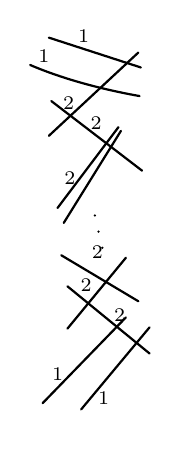
\begin{tikzpicture}[x=.0158cm,y=-.0158cm,line width=.8pt,line cap=round,line join=round,every node/.style={inner sep=0pt,font=\scriptsize}]
\path[use as bounding box] (0,0) rectangle (112,318);
\draw (17,8) -- (91,32);
\draw (2,30) .. controls (30,42) and (62,50) .. (90,55);
\draw (17,87) -- (89,20);
\draw (19,59) -- (92,115);
\draw (24,145) -- (73,80);
\draw (29,157) -- (75,83);
\draw (27,183) -- (89,220);
\draw (32,208) -- (98,262);
\draw (32,242) -- (79,185);
\draw (12,302) -- (79,233);
\draw (43,307) -- (98,241);
\node at (45,7) {$1$};
\node at (13,23) {$1$};
\node at (33,61) {$2$};
\node at (55,77) {$2$};
\node at (34,121) {$2$};
\node at (56,181) {$2$};
\node at (47,207) {$2$};
\node at (74,231) {$2$};
\node at (24,279) {$1$};
\node at (61,298) {$1$};
\fill (54,151) circle[radius=.45pt];
\fill (57,164) circle[radius=.45pt];
\fill (60,177) circle[radius=.45pt];
\end{tikzpicture}}} &
\parbox[c][5.45cm][c]{1.82cm}{\figure{%
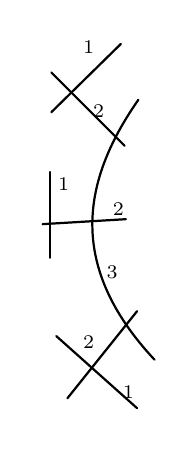
\begin{tikzpicture}[x=.0158cm,y=-.0158cm,line width=.8pt,line cap=round,line join=round,every node/.style={inner sep=0pt,font=\scriptsize}]
\path[use as bounding box] (0,0) rectangle (112,318);
\draw (19,68) -- (75,13);
\draw (19,36) -- (78,95);
\draw (89,58) .. controls (43,124) and (32,192) .. (102,267);
\draw (18,116) -- (18,185);
\draw (12,158) -- (79,154);
\draw (32,298) -- (88,228);
\draw (23,248) -- (88,306);
\node at (49,16) {$1$};
\node at (57,67) {$2$};
\node at (29,126) {$1$};
\node at (73,146) {$2$};
\node at (68,197) {$3$};
\node at (49,253) {$2$};
\node at (81,293) {$1$};
\end{tikzpicture}}} &
\parbox[c][5.45cm][c]{1.82cm}{\figure{%
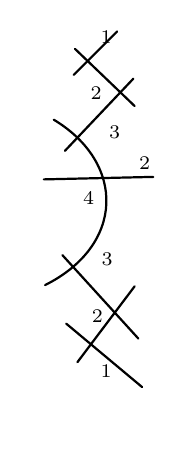
\begin{tikzpicture}[x=.0158cm,y=-.0158cm,line width=.8pt,line cap=round,line join=round,every node/.style={inner sep=0pt,font=\scriptsize}]
\path[use as bounding box] (0,0) rectangle (112,318);
\draw (37,38) -- (72,3);
\draw (38,17) -- (86,63);
\draw (30,99) -- (85,41);
\draw (21,74) .. controls (79,109) and (78,175) .. (14,207);
\draw (13,122) -- (101,120);
\draw (28,183) -- (89,250);
\draw (40,269) -- (86,208);
\draw (31,238) -- (92,289);
\node at (63,8) {$1$};
\node at (55,53) {$2$};
\node at (70,84) {$3$};
\node at (94,109) {$2$};
\node at (49,137) {$4$};
\node at (64,186) {$3$};
\node at (56,232) {$2$};
\node at (63,276) {$1$};
\end{tikzpicture}}} &
\parbox[c][5.45cm][c]{1.82cm}{\figure{%
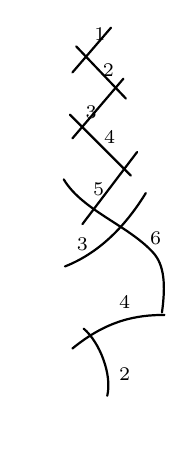
\begin{tikzpicture}[x=.0158cm,y=-.0158cm,line width=.8pt,line cap=round,line join=round,every node/.style={inner sep=0pt,font=\scriptsize}]
\path[use as bounding box] (0,0) rectangle (112,318);
\draw (36,36) -- (67,0);
\draw (39,15) -- (79,57);
\draw (36,89) -- (77,41);
\draw (34,70) -- (83,119);
\draw (44,158) -- (88,100);
\draw (29,122) .. controls (44,147) and (81,159) .. (101,181) .. controls (110,191) and (111,207) .. (108,229);
\draw (30,192) .. controls (58,181) and (79,159) .. (95,133);
\draw (36,258) .. controls (64,235) and (88,231) .. (110,231);
\draw (45,242) .. controls (58,253) and (68,279) .. (64,296);
\node at (58,5) {$\unsure{1}$};
\node at (65,34) {$2$};
\node at (51,68) {$3$};
\node at (66,88) {$4$};
\node at (57,130) {$5$};
\node at (44,174) {$3$};
\node at (103,169) {$6$};
\node at (78,221) {$4$};
\node at (78,279) {$2$};
\end{tikzpicture}}} \\ \hline
\shortstack[l]{$\deleted{\unsure{m|n}}=\,$number of\\irred. components} &
1 & \nu & 1 & 2 & 3 & 5 & 5+\nu & 7 & 8 & 9 \\ \hline
\shortstack[l]{type of group $E(K)/E_0(K)$\\$\approx\widetilde X_0(k)/\widetilde E_0(k)$} &
(1)&(\nu)&(1)&(2)&(3)&(2\times2)&
\substack{(4),\,\nu\ \text{odd}\\2\times2),\,\nu\ \text{even}}&
(3)&(2)&(1)\\ \hline
\widetilde E_0(k)\simeq E_0(K)/E_1(K) &
\widetilde E(k)&k^{*}&k^{+}&k^{+}&k^{+}&k^{+}&k^{+}&k^{+}&k^{+}&k^{+}\\ \hline
\multicolumn{11}{|l|}{\text{S\quad S\quad BELOW THIS LINE THINGS ARE VALID ONLY FOR }\operatorname{CHAR}(k)\ne2,3\quad\text{S}}\\ \hline
v(\Delta_v)&0&\nu&2&3&4&6&6+\nu&8&9&10\\ \hline
\shortstack[l]{$v(\Delta_v)+1-m=f$\\$={}$exp. of $\mathfrak p$ in cond.}&
0&1&2&2&2&2&2&2&2&2\\ \hline
\text{behavior of }j&
v(j)\geq0&
\substack{\deleted{\unsure{v(j)|j}}\\v(j)=-\nu}&
\widetilde j=0&\widetilde j=1728&\widetilde j=0&
v(j)\geq0&v(j)=-\nu&\widetilde j=0&\widetilde j=1728&\widetilde j=0\\ \hline
\end{array}$}}

Here $\widetilde X_0$ denotes the non-singular part of the fiber. This is a (non-connected in general) algebraic group over $k$, whose connected component is $\widetilde E_0$. We have $E(K)/E_1(K)\approx\widetilde X_0(k)$, the isom induced by the reduction map, and assuming now $R$ complete. Note that if $p=\operatorname{char} k\ne2,3$, then we have minimality $\Longleftrightarrow$ \uline{either} $v(\Delta)<12$, \uline{or} $v(\Delta)+v(j)<12$. Also, if $p\ne2,3$, and $f=2$, then $E_0(K)$ is uniquely divisible by $2$ and $3$, while $E(K)/E_0(K)$ is killed by $12$, Hence $E(K)/E_0(K)$ is isomorphic to the group of points in $E(K)$ which are killed by $12$ in \unsure{this}%
\unsure{'|{}}
% archive sheet number: 9
\clearpage

\scanpage{11}\mspage{8.}
7. \uline{Algorithm} \uline{for} \uline{analysing} \uline{singular} \uline{fibers} (\uline{first} \uline{five} \uline{cases}). We assume now that our valuation ring $R$ is \uline{complete}, with \uline{perfect} residual field $k$. In connection with various conjectures, it is well to be able to compute effectively various invariants of an elliptic curve $E$ over $K$, to wit

the \uline{conductor} $f_E={\mathfrak{p}}^{f}$, where $f=v(\Delta)+1-m$, $m$ being the number of components of $\widetilde X$ \uline{over} $\bar k$.

the group $E(K)/E_0(K)$ whose order we denote by $c\deleted{\unsure{.|0}}$

the group $\widetilde E_0(k)$.

To compute these it is necessary to analyse the singular fiber $\widetilde X$ à la Neron, at least when $p=\operatorname{char} k\ne2\text{ or }3$. \reversemarginpar\margin{\figure{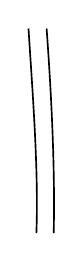
\begin{tikzpicture}[x=1cm,y=1cm]
\draw[line width=.6pt] (0,0) .. controls (.03,.8) and (-.05,1.8) .. (-.10,2.6);
\draw[line width=.6pt] (.22,0) .. controls (.24,.9) and (.18,1.9) .. (.13,2.6);
\end{tikzpicture}}}[If $p=2$ or $3$, everything can be read off the table on page $6$, \deleted{\illegible{1}} if one notes the remarks at the bottom of page $6$; however the algorithm below applies in all cases.] When we refer to the ``\uline{type}'' we mean the type of the singular fiber $\widetilde X$ \uline{over} \uline{the} \uline{algebraic} \uline{closure} $\bar k$ \uline{of} $k$, which is designated by one of the $10$ Kodaira symbols.

To begin with, we simply assume an equation of the form (1.1) with coefficients $\boxed{a_i\in R}$; we do not assume it minimal. If it is not minimal, our algorithm will lead us to a minimalization of it. As we go along we make more and more assumptions. These are \uline{cumulative}, and are \fbox{boxed} for clarity. We include only brief remarks on proofs.

\[
\deleted{\unsure{0|1}}\;\text{\textcircled{1}}\quad
\mathfrak p\nmid\Delta\ \Longrightarrow\ \text{type }\mathrm I_0,\quad
 f=0,\quad c=1,\quad \widetilde E\ \text{\unsure{elliptic}}\,.
\]

\textcircled{2} Assume $\boxed{\mathfrak p\mid\Delta}$. then we can change coordinates so that $\boxed{\mathfrak p\mid a_3,a_4,\text{ and }a_6.}$ Do so. Then $\mathfrak p\nmid b_2\Longrightarrow\text{type }\mathrm I_{\nu}$, with $\nu=v(\Delta)$.

Let $k'$ be the splitting field over $k$ of the congruence $T^2+a_1T-a_2\equiv0$.
\[
\resizebox{\linewidth}{!}{$\displaystyle
\begin{aligned}
\text{\textcircled{\scriptsize 2a}}\;\;k'=k:\qquad&
 f=1,\quad c=v(\Delta),\quad \widetilde E_0(k)\approx k^{*}.\\[.6ex]
\text{\textcircled{\scriptsize 2b}}\;\;k'=k:\qquad&
 f=1,\quad c=\begin{cases}1,&\text{if }v(\Delta)\text{ odd}\\2,&\text{if }v(\Delta)\text{ even}\end{cases},\quad
 \widetilde E_0(k)=\parbox{.23\linewidth}{gp. of elts of $k'$ whose norm to $k$ is $1$.}
\end{aligned}$}
\]

\unsure{Proof}. This case 2) is the one in which $E$ can be described by $\theta$-functions, possibly twisted by an unramified extension. Everything clear from that point of view
\normalmarginpar
% archive sheet number: 10
\clearpage

\scanpage{12}\mspage{9.}
\begingroup
\makeatletter\tagsleft@true\makeatother
From now on $\widetilde E$ has a cusp and $\widetilde E_0(k)=k^+$

\textcircled{3} Assume $\boxed{\mathfrak p\mid b_2}$. Then $\mathfrak p^2\nmid a_6\Longrightarrow\text{type }\mathrm{II}$, and
\[
 f=v(\Delta),\qquad c=1,\qquad \widetilde E_0(k)=k^+.
\]
[Proof. Consider the $2$-dimensional local ring $A=R[x,y]_m$, where $m=(\mathfrak p,x,y)$. It is regular because $a_6\in(x,y)\Rightarrow m=(x,y)$. Hence Weierstrass model $=$ Neron model]

\textcircled{4} Assume $\boxed{\mathfrak p^2\mid a_6}$ (which implies $\mathfrak p^2\mid b_6$ and $b_8$). Then $\mathfrak p^3\nmid b_8\Rightarrow\text{Type }\mathrm{III}$, and
\[
 f=v(\Delta)-1,\qquad c=2,\qquad \widetilde E_0(k)=k^+
\]
\reversemarginpar\margin{\deleted{\unsure{\textcircled{4}|\textcircled{5}}}}[Proof. let $\mathfrak p=\pi R$, and let $a_i=\pi^m a_{i,m}$, $x=\pi^m x_m$, $y=\pi^m y_m$, etc. Our equation can be written
\[
 y_1^2+a_{1,0}x_1y_1+a_{3,1}y_1=\pi x_1^3+a_{2,0}x_1^2+a_{4,1}x_1+a_{6,2}
 \tag*{(7.1)}
\]
The singular point on the fiber (whose local ring was $A$) blows up into the conic
\[
 Y^2+a_{1,0}XY+a_{3,1}Y\equiv a_{2,0}X^2+a_{4,1}X+a_{6,2},
 \tag*{($*$)}
\]
whose descriminant is $b_8\pi^{-2}=b_{8,2}$.]

\textcircled{5} Assume $\boxed{\mathfrak p^3\mid b_8}$ (which implies $\mathfrak p^2\mid b_4$). Then $\mathfrak p^3\nmid b_6\Rightarrow\text{type }\mathrm{IV}$, and
\[
\resizebox{\linewidth}{!}{$\displaystyle\begin{aligned}
 f&=v(\Delta)-2,\quad
 c=\left\{
 \begin{aligned}
 &3\ \text{if}\quad T^2+a_{3,1}T-a_{6,2}\equiv0\quad\text{has roots in }k.\\
 &1\ \text{if}\qquad\qquad\quad \text{''}\qquad\qquad\quad\text{has roots }\notin k
 \end{aligned}\right.,\quad \widetilde E_0(k)=k^+
\end{aligned}$}
\]

[Proof: The conic ($*$) becomes $T^2+a_{3,1}T-a_{6,2}=0$, where $T=Y-\alpha X$ is defined by $(Y-\alpha X)^2\equiv Y^2+a_1XY-a_2X^2$. The discriminant of $T^2+a_{3,1}T-a_{6,2}$ is $\pi^{-2} b_6=b_{6,2}$, so that if $\mathfrak p^3\nmid b_6$, then our conic degenerates into two \uline{distinct} lines. Dividing (7.1) by $x_1^3$, we get an equation of the form $F(U,V)=\pi$, where $F$ is a cubic with coeffs in $R$ which, mod $\pi$, factors into three distinct linear factors, $F\equiv L_1L_2L_3\pmod{\mathfrak p}$, such that the congruences $L_i\equiv0$ have a point in common. The local ring of that point is easily seen to be regular (the max ideal is generated by any two of the three factors $L_i$). Thus (7.1) gives a regular scheme over $R$ with fiber
\parbox[c]{1.48cm}{\setlength{\topsep}{0pt}\figure{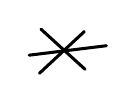
\begin{tikzpicture}[x=1cm,y=1cm,line width=1.1pt,line cap=round]
\draw (-.49,-.07) -- (.49,.05);
\draw (-.34,.26) -- (.22,-.25);
\draw (-.36,-.30) -- (.21,.23);
\end{tikzpicture}}}
consisting of three lines $L_i=0$, $i=1,2,3$ meeting in a point. Concerning the value of $c$, we see that $c$ is equal to the number of these lines which are rational over $k$. One of them is, and the others are given by $T^2+a_{3,1}T-a_{6,2}\equiv0$.
\normalmarginpar
\endgroup
% archive sheet number: 11

\scanpage{13}\mspage{10}
\begingroup
\makeatletter\tagsleft@true\makeatother
8. \uline{Algorithm} \uline{continued}, \uline{the} \uline{last five} \uline{cases}. Assume now that $\boxed{\mathfrak p^3\mid b_6}$. Then we can change coördinates so that $\boxed{\mathfrak p\mid a_1\text{ and }a_2,\quad \mathfrak p^2\mid a_3\text{ and }a_4,\quad \text{and }\mathfrak p^3\mid a_6}$. This being done, consider the polynomial
\[
 P(T)=T^3+a_{2,1}T^2+a_{4,2}T+a_{6,3},
 \tag*{(8.1)}
\]
where the notation is as explained in the proof of step \textcircled{4}, page $9$. Our equation now becomes
\[
 \pi y_2^2+\pi a_{1,1}x_1y_2+\pi a_{3,2}y_2=P(x_1),
 \tag*{(8.2)}
\]
and our algorithm has three branches, according to the multiplicities of the roots of the congruence $P(T)\equiv0$:

\reversemarginpar
\margin{($1^{\mathrm{st}}$ branch)}\textcircled{6} If $P(T)\equiv0$ has three distinct roots, then we have Type $\mathrm I_0^{*}$, and
\[
 f=v(\Delta)-4,\quad\text{and}\quad c=1+(\text{number of roots of }P(T)\equiv0\text{ in }k)
\]

\margin{($2^{\mathrm d}$ branch)}\textcircled{7} If $P(T)\equiv0$ has one simple and one double root, then Type $\mathrm I_{\nu}^{*}$, $\nu>0$, and
\[
 f=v(\Delta)-4-\nu,\qquad c=2\text{ or }4,
\]
where $\nu$ and $c$ are obtained by the following procedure:

\margin{\rotatebox{90}{subprocedure branch \textcircled{7}}%
\figure{\begin{tikzpicture}[x=1cm,y=1cm]
\draw[line width=.8pt,line join=round] (1.25,0) -- (.22,0) -- (.22,-6.2);
\draw[line width=.8pt,line join=round] (.12,-5.94) -- (.22,-6.2) -- (.40,-5.94);
\end{tikzpicture}}}%
Translate $x$, so that $T\equiv0$ is a double root of $P(T)\equiv0$. Then $\mathfrak p^3\mid a_4$, $\mathfrak p^4\mid a_6$, $\mathfrak p^2\nmid a_2$ and (8.2) becomes
\[
 y_2^2+\pi a_{1,1}x_2y_2+a_{3,2}y_2
 =\pi^2x_2^3+\pi a_{2,1}x_2^2+\pi a_{4,3}x_2+a_{6,4}.
 \tag*{\fbox{7.1}}
\]

If $Y^2+a_{3,2}Y-a_{6,4}\equiv0$ has distinct roots, then
\[
 \nu=1,\quad\text{and}\quad c=\begin{cases}4&\text{if roots in }k.\\2&\text{otherwise }.\end{cases}
\]

If $Y^2+a_{3,2}Y-a_{6,2}\equiv0$ has a double root, we can translate $y$ so that the root is $Y\equiv0$. Then $\mathfrak p^3\mid a_3$, $\mathfrak p^5\mid a_6$, and our equation becomes
\[
 \pi y_3^2+\pi a_{1,1}x_2y_3+a_{3,3}y_3
 =\pi x_2^3+a_{2,1}x_2^2+a_{4,3}x_2+a_{6,5}
 \tag*{\fbox{7.2}}
\]

If $a_{2,1}X^2+a_{4,3}X+a_{6,5}\equiv0$ has distinct roots, then
\[
 \nu=2,\ \text{and}\ c=\begin{cases}4&\text{if roots in }k\\2&\text{otherwise}.\end{cases}
\]
\normalmarginpar
\hfill(continued)
\endgroup
% archive sheet number: 12

\scanpage{14}\mspage{\unsure{11|4}.}
\begingroup
\makeatletter
\tagsleft@true
\makeatother
\reversemarginpar
\margin{\raisebox{1.2cm}{\rotatebox{90}{subprocedure branch \textcircled{7}}}\hspace{.15cm}\figure{\begin{tikzpicture}[x=1cm,y=1cm]
\draw[line width=.8pt,line join=round] (.10,-.22) -- (.17,0) -- (.29,-.27);
\draw[line width=.8pt,line join=round] (.17,0) -- (.43,-6.2) -- (2.16,-6.15);
\end{tikzpicture}}}
If $a_{2,1}X^2+a_{4,3}X+a_{6,5}\equiv0$ has double root, then we can translate $x$ so that the root is $X\equiv0$, so that $\mathfrak p^4\mid a_4$ and $\mathfrak p^6\mid a_6$. Equation is now
\[
 y_3^2+\pi a_{1,1}x_3y_3+a_{3,3}y_3
 =\pi^3x_3^3+\pi^2a_{2,1}x_3^2+\pi^2a_{4,4}x_3+a_{6,6}
 \tag*{\fbox{7.3}}
\]

If $Y^2+a_{3,3}\deleted{y}Y-a_{6,6}\equiv0$ has distinct roots, then
\[
 \nu=3,\quad\text{and}\quad c=\begin{cases}
 4&\text{if roots are in }k\\
 2&\text{if not}.
 \end{cases}
\]

If otherwise \unsure{....|:...} etc. Keep going until the quadratic congruence which appears has distinct roots.... The process terminates, because the coefficients $a_3$, $a_4$, and $a_6$ are being made more and more highly divisible by $\mathfrak p$. Hence also $b_4$, $b_6$ and $b_8$, hence also $\Delta$. But $\Delta$ is fixed under all changes of coordinates (translations) involved. A crude estimate gives $\nu\leq\operatorname{ord}\Delta-3$ if I'm not mistaken.

\margin{(branch 3 begins)}\textcircled{8} Suppose now $P(T)\equiv0$ has a triple root. We may assume the root is $T\equiv0$, so $\boxed{\mathfrak p^2\mid a_2,\ \mathfrak p^3\mid a_4,\ \text{and }\mathfrak p^4\mid a_6}$. The equation is
\[
 y_2^2+\pi a_{1,1}x_2y_2+a_{3,2}y_2
 =\pi^2x_2^3+\pi^2 a_{2,2}x_2^2+\pi a_{4,3}x_2+a_{6,4}
 \tag*{\fbox{8.1}}
\]
If $Y^2+a_{3,2}Y-a_{6,4}\equiv0$ has distinct roots, then Type $\mathrm{IV}^{*}$ and
\[
 f=v(\Delta)-6,\qquad c=\begin{cases}3&\text{if roots are in }k\\1&\text{if roots }\notin k.\end{cases}
\]

\margin{(branch 3 continues)}\textcircled{9} Suppose $Y^2+a_{3,2}Y-a_{6,4}\equiv0$ has a double root. Then we can Assume it is $Y\equiv0$, so $\boxed{\mathfrak p^3\mid a_3,\ \mathfrak p^5\mid a_6}$. The equation is now
\[
 \pi y_3^2+\pi a_{1,1}x_2y_3+\pi a_{3,3}y_3
 =\pi x_2^3+\pi a_{2,2}x_2^2+a_{4,3}x_2+a_{6,5}
 \tag*{\fbox{9.1}}
\]
If $a_{4,3}\not\equiv0$, i.e. if $\mathfrak p^4\nmid a_4$, then Type $\mathrm{III}^{*}$, and
\[
 f=v(\Delta)-7\qquad\text{and}\quad c=2
\]

\margin{(branch 3 continues)}\textcircled{\scriptsize 10} Assume $\boxed{\mathfrak p^4\mid a_4}$. Then if $\mathfrak p^6\nmid a_6$ th\deleted{\unsure{a|e|o}}\inserted{e} type is $\mathrm{II}^{*}$ and
\[
 f=v(\Delta)-8\qquad\text{and}\quad c=1.
\]
\normalmarginpar

If $\mathfrak p^6\mid a_6$, original equation was not minimal. Start over with
\[
 y_3^2+a_{1,1}x_2y_3+a_{3,3}y_3=x_2^3+a_{2,2}x_2^2+a_{4,4}x_2+a_{6,6}\quad!
\]
\endgroup
% archive sheet number: 13

\scanpage{16}
\begin{center}
COURBES ELLIPTIQUES : FORMULAIRE

d'après J. Tate\\
mis au goût du jour par P. Deligne
\end{center}

1.\qquad \uline{Formules générales}.

Dans ce formulaire, on appellera courbe de genre $1$ sur un schéma de base $\mathrm{S}$ un morphisme propre et plat de présentation finie
\[
\mathrm{p}:\mathrm{E}\handwritten{\longrightarrow}\mathrm{S}\qquad,
\]
muni d'une section $\mathrm{e}$ contenue dans l'ouvert de lissité, dont les fibres géométriques sont des courbes réduites irréductibles de \handwritten{\uline}{genre arithmétique}\reversemarginpar\margin{\handwritten{?}}\normalmarginpar $1$. Les fibres géométriques de $\mathrm{p}$ sont donc soit :

a) une courbe elliptique, i.e. une courbe propre, lisse et connexe de genre $1$,

b) une droite projective dont on a identifié deux points distincts (cubique dans $\mathrm{P}_{2}$ à point double ordinaire),

c) une droite projective dont on a identifié deux points infiniment voisins (cubique dans $\mathrm{P}_{2}$ à singularité cuspidale).

On dira dans le cas a) (resp. b), c)) que la fibre est de type elliptique (resp. multiplicatif, resp. additif).

Si $\mathrm{E}$ est une courbe de genre $1$ sur $\mathrm{S}$, on définit un faisceau inversible $\omega$ sur $\mathrm{S}$ par la formule
\[
\omega=\mathrm{e}^{*}\,\Omega^{1}_{\mathrm{E}/\mathrm{S}}\qquad.
\]

La section $\mathrm{e}$ est un diviseur de Cartier relatif de $\mathrm{E}$ sur $\mathrm{S}$ ;
% archive sheet number: 15
\clearpage

\scanpage{17}\mspage{- 2 -}
\begingroup
\normalmarginpar
de plus, on vérifie fibre par fibre que
\[
\mathrm{R}^{1}\,\mathrm{p}_{*}\,\handwritten{\mathcal{O}}(\mathrm{ne})=0\quad\text{pour}\quad\mathrm{n}>0\qquad.
\]

Il en résulte, par Riemann-Roch, que pour $\mathrm{n}>0$, le faisceau $\mathrm{p}_{*}\handwritten{\mathcal{O}}(\mathrm{ne})$ est looalement libre de rang $\mathrm{n}$, et que sa formation commute à tout changement de base. La suite exacte de cohomologie fournit de plus une suite exacte
\[
0\handwritten{\longrightarrow}\mathrm{p}_{*}\handwritten{\mathcal{O}}(\mathrm{ne})
\handwritten{\longrightarrow}\mathrm{p}_{*}\handwritten{\mathcal{O}}((\mathrm{n}+1)\mathrm{e})
\handwritten{\longrightarrow}\omega^{\handwritten{\otimes}-(\mathrm{n}+1)}
\handwritten{\longrightarrow}0\quad(\mathrm{n}>0)\,.
\]

Par ailleurs, $\handwritten{\mathcal{O}}(\mathrm{e})$ étant localement libre de rang $1$, on vérifie fibre par fibre, compte tenu de (SGA 1 X 1.2), que
\[
\handwritten{\mathcal{O}}_{\mathrm{S}}\handwritten{\xrightarrow{\sim}}
\mathrm{p}_{*}\handwritten{\mathcal{O}}_{\mathrm{E}}\handwritten{\xrightarrow{\sim}}
\mathrm{p}_{*}\handwritten{\mathcal{O}}(\mathrm{e})\qquad.
\]

En d'autres termes, les $\mathrm{p}_{*}\handwritten{\mathcal{O}}(\mathrm{me})$ pour $1\leq\mathrm{m}\leq\mathrm{n}$ définissent une filtration de $\mathrm{p}_{*}\handwritten{\mathcal{O}}(\mathrm{ne})$, de gradué associé
\makeatletter\tagsleft@true\makeatother
\[
\mathrm{Gr}\;\mathrm{p}_{*}\handwritten{\mathcal{O}}(\mathrm{ne})
=\sum_{\substack{\mathrm{i}=0\\\mathrm{i}\handwritten{\neq}1}}^{\mathrm{n}}\omega^{\handwritten{\otimes}-\mathrm{i}}\qquad.
\tag*{(1.1)}
\]

Le morphisme $\mathrm{p}$ est d'intersection complète relative ; il en résulte que $\mathrm{Rp}^{!}\handwritten{\mathcal{O}}_{\mathrm{S}}\in\mathrm{D}^{+}(\mathrm{E})$ a un seul groupe de cohomologie non\margin{\handwritten{\unsure{réf|vérif|vif}}} nulle, $\mathrm{R}^{1}\,\mathrm{p}^{!}\handwritten{\mathcal{O}}_{\mathrm{S}}$, et que ce dernier est un faisceau inversible sur $\mathrm{E}$ ; on l'appelle le faisceau des différentielles régulières sur $\mathrm{E}$ et on le désigne par $\Omega^{\mathrm{reg}}_{\mathrm{E}/\mathrm{S}}$\margin{\handwritten{$\omega_{\mathrm{E}/\mathrm{S}}$}}. Là où $\mathrm{p}$ est lisse, on a $\Omega^{\mathrm{reg}}_{\mathrm{E}/\mathrm{S}}=\Omega^{1}_{\mathrm{E}/\mathrm{S}}$. La dualité montre que $\mathrm{R}^{1}\mathrm{p}_{*}\Omega^{\mathrm{rcg}}_{\mathrm{E}/\mathrm{S}}$ cst isomorphe à $\handwritten{\mathcal{O}}$, $\mathrm{p}_{*}\Omega^{\mathrm{rcg}}_{\mathrm{E}/\mathrm{S}}$ est donc \handwritten{/} localement libre, de formation compatible à tout changement\margin{\handwritten{réf}} de base et, raisonnant fibre par fibre, on en déduit que
% archive sheet number: 16
\endgroup
\clearpage

\scanpage{18}\mspage{- 3 -}
\begingroup
\makeatletter\tagsleft@true\makeatother
\normalmarginpar
\[
\mathrm{p}_{*}\,\Omega^{\mathrm{reg}}_{\mathrm{E}/\mathrm{S}}\handwritten{\xrightarrow{\sim}}\mathrm{o}^{*}\,\Omega^{1}_{\mathrm{E}/\mathrm{S}}=\omega\quad,
\]
et que pour la flèche adjointe à la flèche inverse
\[
\mathrm{p}^{*}\,\omega\handwritten{\xrightarrow{\sim}}\Omega^{\mathrm{reg}}_{\mathrm{E}/\mathrm{S}}\qquad.
\]
\margin{\handwritten{?}}
Les sections de $\Omega^{\mathrm{reg}}_{\mathrm{E}/\mathrm{S}}$ ainsi associées aux sections de $\omega$ s'appellent les différentielles invariantes.

Soit $\grave{\pi}$ une section inversible de $\omega$ ; il existe, localement pour la topologie de Zariski, une base $(\mathrm{y},\mathrm{x},1)$ de $\mathrm{p}_{*}\handwritten{\mathcal{O}}(3\mathrm{e})$ telle que l'image de $\mathrm{y}$ dans $\omega^{\handwritten{\otimes}-3}$ soit $-\pi^{\handwritten{\otimes}-3}$, que $\mathrm{x}$ appartienne à $\mathrm{p}_{*}\handwritten{\mathcal{O}}(2\mathrm{e})$, et que son image dans $\omega^{\handwritten{\otimes}-2}$ soit $\pi^{\handwritten{\otimes}-2}$. Si $\pi'$ est une autre section inversible de $\omega$, les bases correspondantes s'écrivent toutes, sous forme implicite (pour $\mathrm{r},\mathrm{s},\mathrm{t}$ convenables)
\[
\handwritten{\left\{}\begin{aligned}
\mathrm{x}&=\mathrm{u}^{2}\,\mathrm{x}'+\mathrm{r}\\
\mathrm{y}&=\mathrm{u}^{3}\,\mathrm{y}'+\mathrm{s}\,\mathrm{u}^{2}\,\mathrm{x}'+\mathrm{t}\\
\pi'&=\mathrm{u}\,\pi\qquad.
\end{aligned}\right.
\tag*{(1.2)}
\]

Le faisceau\handwritten{$\backslash$} $\handwritten{\mathcal{O}}(3\mathrm{e})$ est très ample et $(\mathrm{x},\mathrm{y},\rlap{\handwritten{\tikz[overlay,baseline=0pt,x=1em,y=1em]{\draw[thin,gray] (.65,2.45) .. controls (.90,1.50) and (1.05,.75) .. (.66,.20) .. controls (.45,-.45) and (-.28,-.95) .. (-.35,-.58) .. controls (-.47,-.05) and (-.07,1.52) .. (.25,1.65);}}}1)$ sont les coordonnées projectives d'un plongement de $\mathrm{E}$ dans $\mathrm{P}_{2}/\mathrm{S}$.

La courbe image vérifiera une équation
\[
\mathrm{y}^{2}+\mathrm{a}_{1}\,\mathrm{x}\,\mathrm{y}+\mathrm{a}_{3}\,\mathrm{y}
=\mathrm{x}^{3}+\mathrm{a}_{2}\,\mathrm{x}^{2}+\mathrm{a}_{4}\,\mathrm{x}+\mathrm{a}_{6}\qquad.
\tag*{(1.3)}
\]

Pour vérifier l'existence et l'unicité de cette équation, on
\endgroup
% archive sheet number: 17

\scanpage{19}\mspage{- 4 -}
utilise (1.1), en regardant les deux membres de (1.3) comme des sections de $\mathrm{p}_{*}\handwritten{\mathcal{O}}(6\mathrm{e})$ : en effet, $\mathrm{y}^{2}-\mathrm{x}^{3}$ est dans $\mathrm{p}_{*}\handwritten{\mathcal{O}}(5\mathrm{e})$, $\mathrm{xy}$ dans $\mathrm{p}_{*}\handwritten{\mathcal{O}}(5\mathrm{e})$, $\mathrm{x}^{2}$ dans $\mathrm{p}_{*}\handwritten{\mathcal{O}}(4\mathrm{e})$, $\mathrm{y}$ dans $\mathrm{p}_{*}\handwritten{\mathcal{O}}(3\mathrm{e})$, $\mathrm{x}$ dans $\mathrm{p}_{*}\handwritten{\mathcal{O}}(2\mathrm{e})$ et $1$ dans $\mathrm{p}_{*}\handwritten{\mathcal{O}}$.

Si on pose
\[
\mathrm{F}(\mathrm{x},\mathrm{y})=\mathrm{y}^{2}+\mathrm{a}_{1}\,\mathrm{xy}+\mathrm{a}_{3}\,\mathrm{y}-\mathrm{x}^{3}-\mathrm{a}_{2}\,\mathrm{x}^{2}-\mathrm{a}_{4}\,\mathrm{x}-\mathrm{a}_{6}
\]
la forme différentielle invariante définie par $\pi$ s'écrit
\[
\begin{aligned}
\pi&=\mathrm{dx}/\mathrm{F}_{\mathrm{y}}=-\mathrm{dy}/\mathrm{F}_{\mathrm{x}}\qquad\text{soit}\\[.65em]
\pi&=\handwritten{\frac}{\mathrm{dx}}{2\mathrm{y}+\mathrm{a}_{1}\mathrm{x}+\mathrm{a}_{3}}
=\handwritten{\frac}{\mathrm{dy}}{3\mathrm{x}^{2}+2\mathrm{a}_{2}\mathrm{x}+\mathrm{a}_{4}-\mathrm{a}_{1}\mathrm{y}}\qquad.
\end{aligned}
\]

Réciproquement toute équation (1.3) est l'équation non homogène d'une courbe de genre $1$ plongée comme une cubique dans $\mathrm{P}_{2}$ et présentant un point d'inflexion en $(0,1,0)$\margin{\handwritten{$\Big)$\,?}} avec la droite de l'infini pour tangente d'inflexion.

On pose alors
\begingroup
\makeatletter\tagsleft@true\makeatother
\[
\mathrm{b}_{2}=\mathrm{a}_{1}^{2}+4\mathrm{a}_{2}\qquad
\mathrm{b}_{4}=\mathrm{a}_{1}\mathrm{a}_{3}+2\mathrm{a}_{4}\qquad
\mathrm{b}_{6}=\mathrm{a}_{3}^{2}+4\mathrm{a}_{6}
\tag*{(1.4)}
\]
\[
\begin{aligned}
&-\mathrm{b}_{8}=\mathrm{a}_{1}\,\mathrm{a}_{3}\,\mathrm{a}_{4}+\mathrm{a}_{4}^{2}-\mathrm{a}_{1}^{2}\,\mathrm{a}_{6}-\mathrm{a}_{2}\,\mathrm{a}_{3}^{2}-\overset{\inserted{\handwritten{2^{2}}}}{4}\mathrm{a}_{2}\,\mathrm{a}_{6}\\[.55em]
&\mathrm{d}_{6}=\mathrm{b}_{2}\,\mathrm{b}_{4}-\overset{\inserted{\handwritten{2^{1}.3^{2}}}}{18}\mathrm{b}_{6}\qquad
\mathrm{d}_{8}=\mathrm{b}_{2}^{2}\,\mathrm{b}_{4}-2^{4}.3\,\mathrm{b}_{4}^{2}+2.3^{2}\,\mathrm{b}_{2}\,\mathrm{b}_{6}
\end{aligned}
\]
\reversemarginpar\margin{\handwritten{$\unsure{\backslash}$}}\normalmarginpar
\endgroup

On a
\[
\begin{aligned}
&-4\mathrm{b}_{8}=\mathrm{b}_{4}^{2}-\mathrm{b}_{2}\,\mathrm{b}_{6}\\[.45em]
&\rlap{\smash{\handwritten{\tikz[baseline=0pt,x=1em,y=1em]{\draw[thin,gray] (.02,1.32) .. controls (-.22,.65) and (-.42,-.72) .. (-.20,-.92);\draw[thin,gray!65] (-.20,-.92) .. controls (.10,-1.05) and (.67,-.05) .. (.67,.66) .. controls (.67,1.12) and (.55,1.48) .. (.48,1.70);}}}}12\,\mathrm{d}_{6}=\mathrm{c}_{6}+\mathrm{b}_{2}\,\mathrm{c}_{4}\qquad
-\rlap{\smash{\handwritten{\tikz[baseline=0pt,x=1em,y=1em]{\draw[thin,gray!70] (.30,1.14) .. controls (.12,1.39) and (-.26,.20) .. (-.30,-.63);\draw[thin,gray!55] (-.30,-.63) .. controls (-.14,-.93) and (.50,-.10) .. (.64,.70) .. controls (.67,1.02) and (.58,1.35) .. (.54,1.53);}}}}12\,\mathrm{d}_{8}=\mathrm{c}_{4}^{2}+\mathrm{b}_{2}\,\mathrm{c}_{6}
\end{aligned}
\]
\clearpage
% archive sheet number: 18

\scanpage{20}\mspage{- 5 -}
\begingroup
\makeatletter\tagsleft@true\makeatother
\[
\mathrm{c}_{4}=\mathrm{b}_{2}^{2}-\overset{\inserted{\handwritten{2^{3}3}}}{24}\,\mathrm{b}_{4}\qquad
-\mathrm{c}_{6}=\mathrm{b}_{2}^{3}-\overset{\inserted{\handwritten{2^{2}3^{2}}}}{36}\,\mathrm{b}_{2}\,\mathrm{b}_{4}
+\overset{\inserted{\handwritten{2^{3}3^{3}}}}{\rlap{\handwritten{\tikz[overlay,baseline=0pt]{\draw[thin,gray,rotate around={-34:(.78em,.30em)}] (.78em,.30em) ellipse [x radius=1.24em,y radius=1.65em];}}}216}\mathrm{b}_{6}
\tag*{(1.5)}
\]
\[
\begin{aligned}
\Delta&=-\mathrm{b}_{2}^{2}\,\mathrm{b}_{8}-\overset{\inserted{\handwritten{2^{3}}}}{8}\,\mathrm{b}_{4}^{3}
-\overset{\inserted{\handwritten{3^{3}}}}{27}\,\mathrm{b}_{6}^{2}+\overset{\inserted{\handwritten{3^{2}}}}{9}\,\mathrm{b}_{2}\,\mathrm{b}_{4}\,\mathrm{b}_{6}\\[.6em]
&=\mathrm{b}_{4}^{3}-\overset{\inserted{\handwritten{3^{3}}}}{27}\,\mathrm{b}_{6}^{2}
+\mathrm{b}_{8}\bigl(\overset{\inserted{\handwritten{2^{2}3^{2}}}}{36}\,\mathrm{b}_{4}-\mathrm{b}_{2}^{\rlap{\handwritten{\tikz[overlay,baseline=0pt,x=1em,y=1em]{\draw[line width=.4pt,gray] (.18,1.04) .. controls (-.06,.77) and (-.28,.28) .. (-.10,.02) .. controls (.13,-.18) and (.56,-.13) .. (.63,.20) .. controls (.78,.58) and (.54,1.12) .. (.27,1.15);\draw[line width=.4pt,gray] (.27,1.15) .. controls (.14,1.19) and (.08,1.09) .. (.06,1.00);}}}\handwritten{2}}\bigr)\quad\handwritten{\raisebox{.7em}{?}}\quad.
\end{aligned}
\]

Soient maintenant $(\mathrm{x}',\mathrm{y}',\pi')$ reliés à $(\mathrm{x},\mathrm{y},\pi)$ par (1.2). On aura :
\[
\begin{aligned}[t]
\mathrm{u}\,\mathrm{a}'_{1}&=\mathrm{a}_{1}+2\mathrm{s}\\
\mathrm{u}^{2}\,\mathrm{a}'_{2}&=\mathrm{a}_{2}-\mathrm{sa}_{1}+3\mathrm{r}-\mathrm{s}^{2}\\
\mathrm{u}^{3}\,\mathrm{a}'_{3}&=\mathrm{a}_{3}+\mathrm{ra}_{1}+2\mathrm{t}=\mathrm{F}_{\mathrm{t}}(\mathrm{r},\mathrm{t})\\
\mathrm{u}^{4}\,\mathrm{a}'_{4}&=\mathrm{a}_{4}-\mathrm{sa}_{3}+2\mathrm{a}_{2}\mathrm{r}-(\mathrm{t}+\mathrm{rs}){}'\mathrm{a}_{1}+3\mathrm{r}^{2}-2\mathrm{st}
=-\mathrm{F}(\mathrm{r},\mathrm{t})-\mathrm{s}\,\mathrm{F}_{\mathrm{t}}(\mathrm{r},\mathrm{t})\\
\mathrm{u}^{6}\,\mathrm{a}'_{6}&=\mathrm{a}_{6}+\mathrm{ra}_{4}+\mathrm{r}^{2}\mathrm{a}_{2}+\mathrm{r}^{3}-\mathrm{ta}_{3}-\mathrm{t}^{2}-\mathrm{rta}_{1}=-\mathrm{F}(\mathrm{r},\mathrm{t})
\end{aligned}
\tag*{(1.6)}
\]
\[
\begin{aligned}[t]
\mathrm{u}^{2}\,\mathrm{b}'_{2}&=\mathrm{b}_{2}+12\,\mathrm{r}\\
\mathrm{u}^{4}\,\mathrm{b}'_{4}&=\mathrm{b}_{4}+\mathrm{rb}_{2}+6\mathrm{r}^{2}\quad(\text{équ. de discr. }\mathrm{c}_{4})\\
\mathrm{u}^{6}\,\mathrm{b}'_{6}&=\mathrm{b}_{6}+2\mathrm{r}\,\mathrm{b}_{4}+\mathrm{r}^{2}\,\mathrm{b}_{2}+4\mathrm{r}^{3}\quad(\text{équ. de discr. }16\,\Delta)\\
\mathrm{u}^{8}\,\mathrm{b}'_{8}&=\mathrm{b}_{8}+3\mathrm{r}\,\mathrm{b}_{6}+3\mathrm{r}^{2}\,\mathrm{b}_{4}+\mathrm{r}^{3}\,\mathrm{b}_{2}+3\mathrm{r}^{4}\\
\mathrm{u}^{6}\,\mathrm{d}'_{6}&=\mathrm{d}_{6}+\mathrm{c}_{4}\,\mathrm{r}\qquad\mathrm{u}^{8}\,\mathrm{d}'_{8}=\mathrm{d}_{8}-\mathrm{c}_{6}\,\mathrm{r}
\end{aligned}
\tag*{(1.7)}
\]
\endgroup
% archive sheet number: \unsure{13|19}
